\documentclass[tikz, margin=3.14mm]{standalone}

\usepackage{tikz}
\usepackage{graphics}
\usepackage{amsmath, amsfonts, amssymb, mathrsfs}

\usetikzlibrary{shapes.geometric, positioning, shapes}

\begin{document}
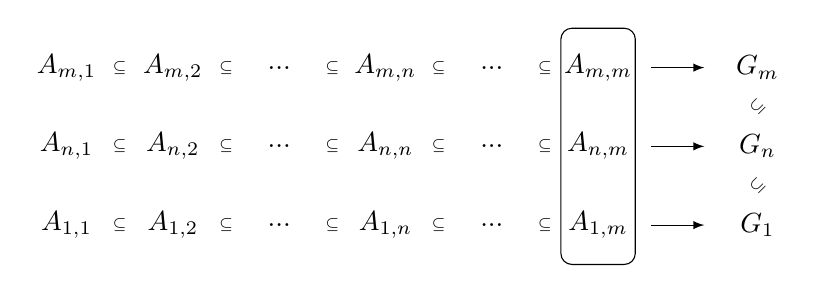
\begin{tikzpicture}[yscale=1, xscale=1.35]
    \node at (2, 0) {$A_{m,1}$};
    \node at (2.5,0) {\tiny$\subseteq$};
    \node at (3, 0) {$A_{m,2}$};
    \node at (3.5,0) {\tiny$\subseteq$};
    \node at (4, 0) {$...$};
    \node at (4.5,0) {\tiny$\subseteq$};
    \node at (5, 0) {$A_{m,n}$};
    \node at (5.5, 0) {\tiny$\subseteq$};
    \node at (6, 0) {...};
    \node at (6.5, 0) {\tiny$\subseteq$};
    \node at (7, 0) {$A_{m,m}$};

    \node at (2, -1) {$A_{n,1}$}; 
    \node at (2.5, -1) {\tiny$\subseteq$};
    \node at (3, -1) {$A_{n,2}$};
    \node at (3.5, -1) {\tiny$\subseteq$};
    \node at (4, -1) {$...$};
    \node at (4.5, -1) {\tiny$\subseteq$};
    \node at (5, -1) {$A_{n,n}$};
    \node at (5.5, -1) {\tiny$\subseteq$};
    \node at (6, -1) {...};
    \node at (6.5, -1) {\tiny$\subseteq$};
    \node at (7, -1) {$A_{n,m}$};

    \node at (2, -2) {$A_{1,1}$};
    \node at (2.5, -2) {\tiny$\subseteq$};
    \node at (3, -2) {$A_{1,2}$};
    \node at (3.5, -2) {\tiny$\subseteq$};
    \node at (4, -2) {$...$};
    \node at (4.5, -2) {\tiny$\subseteq$};
    \node at (5, -2) {$A_{1,n}$};
    \node at (5.5, -2) {\tiny$\subseteq$};
    \node at (6, -2) {...};
    \node at (6.5, -2) {\tiny$\subseteq$};
    \node at (7, -2) {$A_{1,m}$};

    \draw [-latex] (7.5, 0) -- (8, 0);
    \draw [-latex] (7.5, -1) -- (8, -1);
    \draw [-latex] (7.5, -2) -- (8, -2);

    \node at (8.5, 0) {$G_m$};
    \node at (8.5, -1) {$G_n$};
    \node at (8.5, -2) {$G_1$};

    \node at (8.5, -0.5) {\tiny\rotatebox{45}{$\subseteq$}};
    \node at (8.5, -1.5) {\tiny\rotatebox{45}{$\subseteq$}};

    % rounded corner rectangle around the A_{m,m}, A_{n,m}, A_{1,m} column
    \draw [rounded corners] (6.65, 0.5) -- (7.35, 0.5) -- (7.35, -2.5) -- (6.65, -2.5) -- cycle;

\end{tikzpicture}
\end{document}